% marc.tex — MARC paper draft (corrected framing; every number traces to paper/RESULTS.md)
\documentclass[11pt]{article}
% swap for aaai2026.sty + authblk config before submission
\usepackage[margin=1in]{geometry}
\usepackage{amsmath,amssymb}
\usepackage{booktabs}
\usepackage{graphicx}
\usepackage{natbib}
\usepackage[hidelinks]{hyperref}

\title{Learn the Structure, Not the Values:\\
A Controlled Characterization of Learning in Exact Constraint Solving}
% author block: team fills in names, order, and affiliations before submission
\author{...}
\date{}

\begin{document}
\maketitle

\begin{abstract}
Learned proposals for constraint solving are usually evaluated against cold-start refinement;
the control that matters is random multi-start at the same budget. We run that control on our
own system and our headline claim shrinks. MARC poses continuous algebraic systems as factor
graphs, proposes values with a graph diffusion model, polishes them on exact computer-algebra
energies, and accepts only what an exact symbolic checker verifies. Under this protocol,
learned value proposals help only where acceptance basins factorize across variables and
dimension defeats random search ($0.975$ versus $0.075$ at $n{=}3$); a parameter-free law in
the measured single-start reachability reproduces the full restart curve (MAE $0.012$),
predicts the failure under variable coupling, and holds on eight named real systems, where
classical multi-start leaves no learning-favorable regime. The decision that has no classical
baseline is discrete: which structural augmentation repairs an unsolvable system. A
candidate-conditioned ranker chooses repairs on certificate-grade menus --- ``exactly one
solvable option'' is a computer-algebra theorem, not a budget-relative claim --- at $0.997$
versus $0.236$ random ($p<10^{-70}$, seed-robust), beating budget-matched per-candidate probes
on accuracy and cost together. Every negative result is reported with confidence intervals;
they are the boundary of the claim. Learning earns its keep on the structural decision;
everything else belongs to the solvers.
\end{abstract}

\section{Introduction}
\label{sec:intro}

Solving a system of algebraic constraints involves two different kinds of decision. The
continuous decision asks which values satisfy the equations; it is smooth, gradient-rich, and
has been owned by numerical analysis for sixty years. The discrete decision asks which
representation makes the problem tractable at all: which auxiliary variable, substitution, or
defining relation to introduce. Classical solvers have nothing to say about the second
decision, and for the first they are very hard to beat. This paper measures, under controlled
conditions, whether a learned diffusion model helps with the value decision on continuous
algebraic constraint systems. The short answer is: only in a narrow regime, and we can say
exactly which one.

The measurement matters because the comparison usually reported is the wrong one. A learned
proposal followed by refinement is typically compared against refinement from a cold start,
and it wins. That comparison conflates two effects: the value of starting refinement from
diverse initializations, and the value of the learned model specifically. The control that
separates them is random multi-start with the same polish and the same candidate budget. When
we added that control, our own headline claim shrank, and the corrected claim is the subject
of this paper.

Our system, MARC, is an orchestrator rather than a solver. A problem is represented as a
factor graph over variables and symbolic constraint expressions. A graph neural network
trained as a diffusion denoiser proposes candidate assignments. Classical machinery finishes
the job: an exact computer-algebra system (CAS) supplies residuals, an energy, and its
gradient; deterministic energy descent polishes each proposal; and a two-stage checker
(numeric gate, then exact symbolic verification after snapping to rationals) is the sole
acceptance criterion. Nothing counts as solved unless the checker says so. The design follows
the division of labor that AlphaGeometry demonstrated in geometry \citep{trinh2024alphageometry}:
neural proposals for decisions that admit no gradient, symbolic engines for everything they
already do well.

Within that architecture we ask a specific question. When does the learned proposal earn its
place over the classical alternatives? We evaluate against a graded battery: deterministic
energy descent, annealed Langevin descent, a mean-prior control that starts polish from the
training-distribution mean, and random multi-start with identical polish and budget. The
answer has three parts. On non-convex families where deterministic descent is fully trapped,
any diverse proposal plus polish beats cold-start Langevin; the learned proposal ties or loses
to random restart on all four families, so the hybrid recipe is the useful result there
(Section~\ref{sec:hybrid}). On bundled trap families with wide, per-instance-varying roots,
there is a clean crossover at $n = 3$: random restart wins at low dimension, collapses once it
must hit all $n$ basins by chance, and the learned proposal holds where it fails
(Section~\ref{sec:scaling}). On coupled chained-bilinear systems, where the solution is a
joint object rather than a product of per-variable marginals, the learned advantage vanishes:
the learned proposal ties or loses to random restart at every dimension we tested, with zero
significant wins in five comparisons (Section~\ref{sec:coupled}).

We therefore claim a characterization, not a victory. Learned diffusion proposals amortize
independent search: they help when solutions are per-variable separable and the dimension
defeats random restart, and this advantage disappears under coupling. Section~\ref{sec:law}
states the characterization as a parameter-free law in the measured single-start reachability
and validates it on both synthetic families and a geometric domain. Alongside this we
contribute the substrate itself (factor graphs with an exact CAS and an exact accept checker
in the loop), a pre-registered entrapment result showing that annealed noise escapes
deterministic traps with a confidence interval that excludes zero, a partial cross-family
transfer result, and a scope measurement on the MATH benchmark showing that autoformalization,
not solving, is the binding constraint. We make no claim against combinatorial-optimization
solvers such as DIFUSCO; the problem class is different (Section~\ref{sec:related}). Every
rate we report carries $N$ and a 95\% Wilson interval or a $z$-test, and the negative results
are reported in full because they are the boundary of the claim.

\section{Related Work}
\label{sec:related}

\paragraph{Multistart global optimization.}
The classical parts of our factorization law are classical. Best-of-$K$ multistart succeeds
with probability $1-(1-q)^K$ in the single-start reachability $q$, and basin structure governs
the cost of stochastic global search \citep{rinnooykan1987clustering,
rinnooykan1987multilevel}; that annealed noise escapes minima where descent stalls is likewise
textbook \citep{welling2011sgld, bras2021langevin, regularized2025langevin}, and our
entrapment experiment (Section~\ref{sec:entrapment}) is confirmation on this substrate, not
novelty. What we add is the diagnostic, not the $v^n$ basin count: the measured $\log q(n)$
slope, one constant that reproduces the best-of-8 restart curve parameter-free (MAE 0.012),
and the two-condition dissection --- collapse \emph{and} separability --- deciding when a
learned proposal can beat the multistart bound at all.

\paragraph{Learned initialization and amortized optimization.}
A model that maps a problem instance to a solver starting point is a learned warm start:
\citet{amos2023amortized} surveys amortized optimization, learned starts accelerate AC
optimal power flow \citep{baker2019warmstart}, reinforcement learning tunes QP solvers
\citep{ichnowski2021rlqp}, and amortized Langevin inference \citep{taniguchi2022langevin} and
diffusion proposals with bootstrapped refinement \citep{bootstrapped2025refinement} are the
nearest neural instances, replacing search whose cost grows like $v^{-n}$ with dimension.
This is the literature our value-proposal negative indicts. Its standard evaluation compares
a learned start against a cold start; under random multistart at the same refinement budget
--- a control this line does not run on itself --- our own proposal's advantage survives only
where solutions factorize per variable and dimension defeats random search.

\paragraph{Learning for combinatorial optimization.}
Two branches of neural CO border this work: graph diffusion solvers for NP-complete problems
--- DIFUSCO \citep{sun2023difusco} and its unsupervised \citep{sanokowski2024diffuco},
trajectory \citep{li2024constraintaware}, and vehicle-routing \citep{anon2026vrpdiffusion}
successors --- and learning-to-branch, from strong-branching surrogates \citep{khalil2016branch}
to bipartite-GNN branching \citep{gasse2019exact}, surveyed by \citet{bengio2021mlco}. MARC
differs in problem class and in where the verifier sits: continuous algebraic systems, an
exact CAS supplying residuals, gradients, and the sole acceptance checker, and a learned
discrete decision that is a pre-solve repair of the constraint graph, not branching inside a
search tree. We do not compete on their benchmarks; neither branch reports the
budget-matched multistart control this study is built around.

\paragraph{Per-instance algorithm selection.}
The repair ranker of Section~\ref{sec:repair} is, at bottom, per-instance selection: given an
instance and $K$ discrete options, pick the one under which a downstream solver succeeds. The
problem statement is fifty years old \citep{rice1976algorithm}, SATzilla made per-instance
portfolio selection standard practice \citep{xu2008satzilla}, and \citet{kerschke2019survey}
survey the field; AlphaGeometry \citep{trinh2024alphageometry} is the precedent for learning
the structural decision itself, and discrete diffusion \citep{austin2021d3pm,
vignac2023digress} supplied the formalism for our withdrawn predecessor policy. Three things
in Section~\ref{sec:repair} are not in this line: certificate-grade menu semantics (``exactly
one solvable option'' is a CAS theorem, not a budget-relative claim), candidate conditioning
(the ranker encodes each candidate-augmented graph, not instance features alone), and
controls that price the classical recourse --- budget-matched restarts and a per-candidate
solver probe --- rather than a single default algorithm.

\paragraph{Distance geometry.}
The geometric family of Section~\ref{sec:law} --- chains of points pinned by squared-distance
constraints --- is a distance geometry problem with known discrete structure: each new point
lies on an intersection of circles, the per-point reflection ambiguity is the discrete branch
that branch-and-prune enumerates, and the solution set carries a group of partial reflections
\citep{lavor2012dmdgp, liberti2014distance}. We claim none of that structure; the ambiguities
our reachability measurement counts are exactly those branches. What we add is measurement
under shared machinery: the reachability slope under one fixed polish ($-0.77$), the finding
that a trained proposal ties restart-matched random search there anyway, and --- where
learning enters the branches through structural repair --- selection learned from measured
labels under restart-matched controls; the branch vocabulary is this literature's.

\section{Method}
\label{sec:method}

\subsection{Constraint graphs and the exact symbolic layer}

A problem instance is a factor graph $G = (V, F)$ with variable nodes $V = \{x_1, \dots,
x_n\}$ and factor nodes $F = \{g_1, \dots, g_m\}$, each factor carrying a symbolic expression
string. A bare expression $g$ denotes the equality $g = 0$; relational expressions denote
non-strict inequalities. The residual of factor $j$ at assignment $x$ is $r_j(x) = |g_j(x)|$
for equalities and the hinge $\max(0, g_j(x))$ for inequalities, so $r_j(x) = 0$ exactly when
the constraint holds. The energy is
\begin{equation}
E(x) \;=\; \tfrac{1}{2} \sum_{j=1}^{m} r_j(x)^2 .
\end{equation}
Residuals, energy, and $\nabla E$ are computed exactly by a CAS (SymPy) and compiled once per
graph. Acceptance is a two-stage gate: a numeric stage rejects fast if any factor's violation
exceeds a tolerance, and a symbolic stage snaps the candidate to nearby exact rationals and
re-checks every constraint exactly. The symbolic stage is authoritative; it catches
false accepts that a numeric tolerance admits. The checker is the only acceptance criterion in
every experiment and the only reward source in training.

\subsection{The learned proposal: a GNN denoiser with guided reverse diffusion}

The forward process is standard Gaussian diffusion over variable values with a cosine noise
schedule over $T = 1000$ steps. The denoiser is a bipartite message-passing GNN: variable
nodes are encoded from their current noisy value and type, factor nodes from their type, their
residual at the current values, and a sinusoidal timestep embedding; $L$ rounds of bipartite
message passing are followed by a per-variable head that predicts the noise
$\hat{\varepsilon}$. Sampling runs DDIM reverse steps with energy-gradient guidance,
\begin{equation}
\hat{s} \;=\; s_\theta(x_t, t, G) \;-\; \lambda_t \nabla E(x_t),
\end{equation}
where $s_\theta$ is the score implied by the predicted noise ($s_\theta \propto
-\hat{\varepsilon}$ under the standard Gaussian identity); the exact CAS gradient steers the
reverse process toward feasibility.

One architectural detail proved necessary. Message passing applies LayerNorm each round, which
washes out the magnitude of constraint constants, so a variable whose value is pinned by its
own constraint cannot be read off the deep features. A direct linear skip from a variable's
incident-factor constants to its output restores the path and cut the mean absolute root error
from 5.4 to 0.9. We report this because it is the kind of failure that silently caps a
graph-network solver's numerical capacity.

\subsection{Propose and polish, and the baseline battery}

The system solver is a hybrid. The diffusion model proposes $K$ candidate assignments
(best-of-8 throughout); each is polished by deterministic descent on $E$; the first candidate
to pass the checker is the answer. The baselines are graded so that each isolates one
ingredient. Deterministic energy descent from a cold start is the plain relaxation
\begin{equation}
x^{(k+1)} \;=\; x^{(k)} - \eta \, \nabla E\!\left(x^{(k)}\right) + \sigma_k \xi_k,
\qquad \xi_k \sim \mathcal{N}(0, I),
\end{equation}
with $\sigma_k \equiv 0$; it stalls at points where $\nabla E = 0$ but $E > 0$. Annealed
Langevin descent sets $\sigma_k$ on a decreasing schedule and is the classical stochastic
solver. The mean-prior control starts polish from the training-distribution mean and tests
whether the learned model does more than reproduce an average solution. The decisive control
is random multi-start: $K$ initializations drawn uniformly from a family-matched box covering
the root range ($[-5,5]^n$ on the Section~\ref{sec:hybrid} families, $[-8,8]^n$ on the
dimension-scaling traps, $[-4,4]^n$ on the coupled chains), polished identically, same budget,
no learning. Throughout the paper \emph{refine}, \emph{random}, and
their variants are labeled classical baselines; the learned hybrid is the system.

MARC as a whole is an orchestrator built from these parts: learned components propose,
classical solvers finish, and the checker decides. The experiments below measure which
decisions the learned component actually improves.

\section{Experiments}
\label{sec:experiments}

\subsection{Protocol}

All problem families are procedurally generated with held-out test instances. Unless stated
otherwise, solve rates are best-of-8 over $N = 60$ held-out instances per family, intervals
are 95\% Wilson intervals, and comparisons are one-sided two-proportion $z$-tests of
learned $>$ baseline, so identical proportions read as $p = 0.50$. Before any
comparison we verified that the learned solver converges at all: after five implementation
faults were found and fixed (the denoiser never received $x_t$; constants were absent from the
graph tensors; $t$ did not condition variable nodes; guidance magnitudes exploded; a
shape-handling fault in the one-variable case), the solve rate on convex linear systems went
from 0 to 1.000 both in-distribution and held out, with a generalization gap of zero. Convex
families are saturated by every method and carry no comparative signal; all results below are
on non-convex families.

\subsection{Entrapment: noise escapes where deterministic descent cannot}
\label{sec:entrapment}

We pre-registered the question of whether annealed noise reduces entrapment, with
falsification defined as no reduction. On 200 non-convex problems, deterministic energy
descent is trapped on every instance; annealed Langevin descent cuts the entrapment rate to
0.475 (Table~\ref{tab:entrapment}). The reduction is $0.525 \pm 0.086$ and the 95\% interval
excludes zero ($N = 200$, 5 seeds). This is textbook annealed-Langevin behavior and we present
it as a confirmed premise for everything that follows, not as a novel finding: stochasticity
matters in this search space, whether or not the noise source is learned.

% provenance: RESULTS.md R2
\begin{table}[t]
\centering
\caption{Entrapment on 200 non-convex problems ($N = 200$, 5 seeds). Reduction
$0.525 \pm 0.086$; the 95\% CI excludes 0.}
\label{tab:entrapment}
\begin{tabular}{lc}
\toprule
Solver & Entrapment rate \\
\midrule
Deterministic energy descent & 1.000 \\
Annealed Langevin descent    & 0.475 \\
\bottomrule
\end{tabular}
\end{table}

\subsection{The hybrid recipe: a good proposal plus polish beats cold-start refinement}
\label{sec:hybrid}

Table~\ref{tab:hybrid} shows the mechanism ablation on four non-convex families where
deterministic descent is fully trapped (best-of-8, 60 held-out instances per family, 95\%
Wilson intervals). Cold-start refinement solves nothing; adding Langevin noise helps somewhat;
and both the random-init control and the learned hybrid do far better. The comparison that
matters is the last column. The learned proposal ties random multi-start on two families
($p = 0.50$) and loses on two, including a complete failure on CircleLine (0.000 where random
reaches 0.200).

% provenance: RESULTS.md R3
\begin{table}[t]
\centering
\caption{Mechanism ablation on trapped non-convex families (best-of-8, 60 held-out per
family, 95\% Wilson CIs). The random-init control uses identical polish and budget with no
learning.}
\label{tab:hybrid}
\footnotesize
\begin{tabular}{lccccl}
\toprule
Family & refine cold & refine+Langevin & random-init+polish & learned hybrid & learned $>$ random? \\
\midrule
BilinearSystem  & 0.000 & 0.300 & 0.550 [0.42, 0.67] & 0.550 & tie ($p = 0.50$) \\
BilinearProduct & 0.000 & 0.100 & 0.717 [0.59, 0.81] & 0.683 & no (random wins) \\
QuadraticSystem & 0.000 & 0.300 & 0.683 [0.56, 0.79] & 0.683 & tie ($p = 0.50$) \\
CircleLine      & 0.000 & 0.033 & 0.200 [0.12, 0.32] & 0.000 & no (random wins) \\
\bottomrule
\end{tabular}
\end{table}

This corrects an earlier over-claim of ours. Without the random control, the table reads as
``the learned solver beats classical refinement''; with it, the correct reading is that
diverse restarts plus deterministic polish beat cold-start Langevin, and the learned proposal
adds nothing on these families. The reason is unglamorous: solutions here are small integers
in $[-3,3]$, which random restart over $[-5,5]$ hits readily, so there is nothing for learning
to amortize. The hybrid recipe is the useful result; the denoiser is not.

\subsection{Cross-family transfer is partial}
\label{sec:transfer}

We train on three non-convex families and test the hybrid on the held-out fourth (best-of-8,
60 test instances per family, 200 epochs). Table~\ref{tab:transfer} reports the outcome. On
two of four held-out families the cross-trained model reaches 0.683, significantly above the
refine+Langevin baseline ($p < 10^{-4}$): the model solves a family it never trained on. On the
other two it solves nothing. The BilinearSystem failure is the informative one, because that
family is solvable in-distribution (0.550 in Table~\ref{tab:hybrid}). A smoke run trained on
only the two similar families \{Product, Quadratic\} recovered it at 0.70, whereas adding the
pathological CircleLine family to the training mix collapsed it to 0.00. Dissimilar training
families can actively disrupt transfer. We read this as transfer across related non-convex
structure, not as a universal solver.

% provenance: RESULTS.md R4
\begin{table}[t]
\centering
\caption{Leave-one-family-out transfer (best-of-8, 60 test per family, 200 epochs). $p$ from a
$z$-test of learned (cross) $>$ refine+Langevin.}
\label{tab:transfer}
\small
\begin{tabular}{lllll}
\toprule
Held-out family & Trained on & refine+Langevin & learned (cross) & $p$ \\
\midrule
BilinearProduct & Sys, Quad, Circle  & 0.100 [0.05, 0.20] & 0.683 [0.56, 0.79] & $<10^{-4}$ \\
QuadraticSystem & Sys, Prod, Circle  & 0.300 [0.20, 0.43] & 0.683 [0.56, 0.79] & $<10^{-4}$ \\
BilinearSystem  & Prod, Quad, Circle & 0.300 [0.20, 0.43] & 0.000 & fails \\
CircleLine      & Sys, Prod, Quad    & 0.033 [0.01, 0.11] & 0.000 & fails \\
\bottomrule
\end{tabular}
\end{table}

\subsection{Dimension scaling: the crossover where learning earns its keep}
\label{sec:scaling}

The families in Section~\ref{sec:hybrid} give random restart an easy target. To test the
amortization argument we use bundled non-convex traps whose roots vary per instance over a
wide signed range ($\pm[3,8]$), so neither a fixed prior nor a lucky draw suffices.
Table~\ref{tab:scaling} shows solve rates by dimension with the full battery, including the
random multi-start control at the same best-of-8 budget.

% provenance: RESULTS.md R15 (methodology unified-v2, results/p_scaling/scaling.json)
\begin{table}[t]
\centering
\caption{Dimension scaling on bundled traps with per-instance-varying roots in $\pm[3,8]$
(best-of-8, unified-v2 protocol: one shared polish and one checker for every arm, $N{=}40$
per cell). Bold marks the best method per row.}
\label{tab:scaling}
\begin{tabular}{cccccc}
\toprule
$n$ & deterministic & Langevin & mean-prior & random restart & learned \\
\midrule
1 & 0.000 & 0.775 & 0.000 & \textbf{1.000} & 0.950 \\
2 & 0.000 & 0.225 & 0.000 & 0.725 & \textbf{0.950} \\
3 & 0.000 & 0.000 & 0.000 & 0.075 & \textbf{0.975} \\
4 & 0.000 & 0.000 & 0.000 & 0.000 & \textbf{0.925} \\
6 & 0.000 & 0.000 & 0.000 & 0.000 & \textbf{0.250} \\
\bottomrule
\end{tabular}
\end{table}

There is a clean crossover by $n = 3$. At $n = 1$ random restart wins (1.000 against 0.950):
the solution space is small enough to brute-force and learning buys nothing. From
$n = 3$ random restart collapses (0.075, then 0.000), because a random initialization must
land in all $n$ basins simultaneously: the probability of that event decays like $v^n$ in the
per-variable reachability $v$, so the restart cost grows like $v^{-n}$
(Section~\ref{sec:law}). The learned
proposal holds essentially flat where random fails: 0.975 at $n = 3$ and 0.925 at $n = 4$ ---
the flat learned ceiling the law of Section~\ref{sec:law} takes as its input. Langevin and the
mean-prior are at or near zero from $n = 3$. This is the amortized-inference result: a
per-instance learned proposal replaces a search whose cost is exponential in dimension. Two
caveats bound it. The learned model degrades at $n = 6$ (0.250), and random restart is at
ceiling at $n = 1$. The claim is that the amortized proposal beats random search in high
dimension, and only there.

Two natural objections are that this is one designed family and that random multi-start is a
weak baseline. We answer both by rerunning the experiment on three structurally different
separable families (varying the spurious-well shape and the root range) with an added
Levenberg--Marquardt arm (analytic Jacobian, eight Gaussian multistarts).
% provenance: RESULTS.md R27 + PROVENANCE R27 (crossover_families.json)
Levenberg--Marquardt is not a way out: multi-start LM must also hit all $n$ independent basins,
so it collapses along the same geometric $v^n$ curve (baseline LM $0.825, 0.575, 0.200, 0.100, 0.000$ at
$n = 1, 2, 3, 4, 6$). On two of the three families the learned proposal significantly beats
\emph{both} random restart and LM at high dimension (on the baseline family, learned $1.000$
against $0.000$ for both at $n = 6$; on the wide-root family, $0.225$ against $0.000$ for both at
$n = 4$). The crossover is therefore a property of separable structure, not of one construction,
and it holds against the strong classical solver, not only against random search. On the third
family (two spurious wells) the small denoiser did not learn the harder marginals and collapsed
with the classical methods, which sharpens the boundary: learning wins only where it can actually
amortize the per-variable marginals.

\subsection{A factorization law predicts both results}
\label{sec:law}

The crossover above and the coupled negative reported next are two outcomes of one mechanism,
and the mechanism can be stated as a law and tested without fitting anything. Every method in
this study shares one polish operator and one acceptance checker; methods differ only in where
they start the polish. For a problem instance, define the single-start reachability
% provenance: RESULTS.md R9 + paper/notes/crossover_law.md §1
\begin{equation}
q(n) \;=\; \Pr_{x_0 \sim U}\big[\,\text{polish}(x_0)\ \text{is accepted}\,\big],
\end{equation}
the probability that one random start, pushed through the shared polish, lands in an accepting
basin. This is a geometric property of the problem family and the polish operator, with no
learning in it. Random multi-start with budget $K$ succeeds iff at least one of $K$ i.i.d.\
starts is accepted, so
% provenance: RESULTS.md R9 + paper/notes/crossover_law.md §2
\begin{equation}
P_{\text{random}}(n;K) \;=\; 1 - \big(1 - q(n)\big)^{K} .
\label{eq:bestofk}
\end{equation}
The identity is exact for a fixed instance; across a family we use the instance-averaged
version, with per-instance heterogeneity a second-order correction
(Section~\ref{sec:limitations}). It already says that a hybrid beating cold-start Langevin has
proven nothing about the value of learning: it must beat Eq.~\eqref{eq:bestofk} at the same
$K$.

How $q(n)$ scales with dimension is decided by whether the acceptance basins factorize across
variables. If each factor touches one variable, as in the bundled trap family, the polish is
coordinate-decoupled and a start is accepted only when every coordinate independently lands in
its root basin, so $q(n) = v^n$ with $v := q(1)$: $\log q$ is linear in $n$, reachability
decays geometrically, and random search needs $\Theta(v^{-n})$ starts to hold a fixed success
rate. If factors couple variables, as in the chained bilinear family, the solution is a joint
object, the polish propagates corrections along the chain, and $q(n)$ need not decay
geometrically at all. We measured $q(n)$ directly by single-start polish on 600 fresh
instances per $n$ (Wilson intervals), with the same generators, polish, and checker as the
solve-rate experiments. Table~\ref{tab:law} shows the dichotomy.

% provenance: RESULTS.md R9 + paper/notes/crossover_law.md §5
\begin{table}[t]
\centering
\caption{The factorization dichotomy, measured (600 fresh instances per $n$, Wilson CIs,
$K = 8$). Expected restarts $1/q(n)$ are listed over the tested dimensions in increasing
order.}
\label{tab:law}
\small
\begin{tabular}{lll}
\toprule
Quantity & Independent (separable) & Coupled \\
\midrule
$\log q(n)$ slope & $-1.03$ & $-0.13$ \\
fit $R^2$ & 0.98 & 0.96 \\
measured $v = q(1)$ & 0.27 & --- \\
$E[\text{starts}] = 1/q(n)$ & $3.7 \to 13 \to 32 \to 150 \to 600$ & $2.0 \to 2.5 \to 2.9 \to 3.8 \to 4.3$ \\
$P_{\text{random}}$ MAE, parameter-free & 0.012 & law N/A (not separable) \\
\bottomrule
\end{tabular}
\end{table}

% provenance: paper/figures/fig_crossover_theory.pdf, RESULTS.md R9
\begin{figure}[t]
\centering
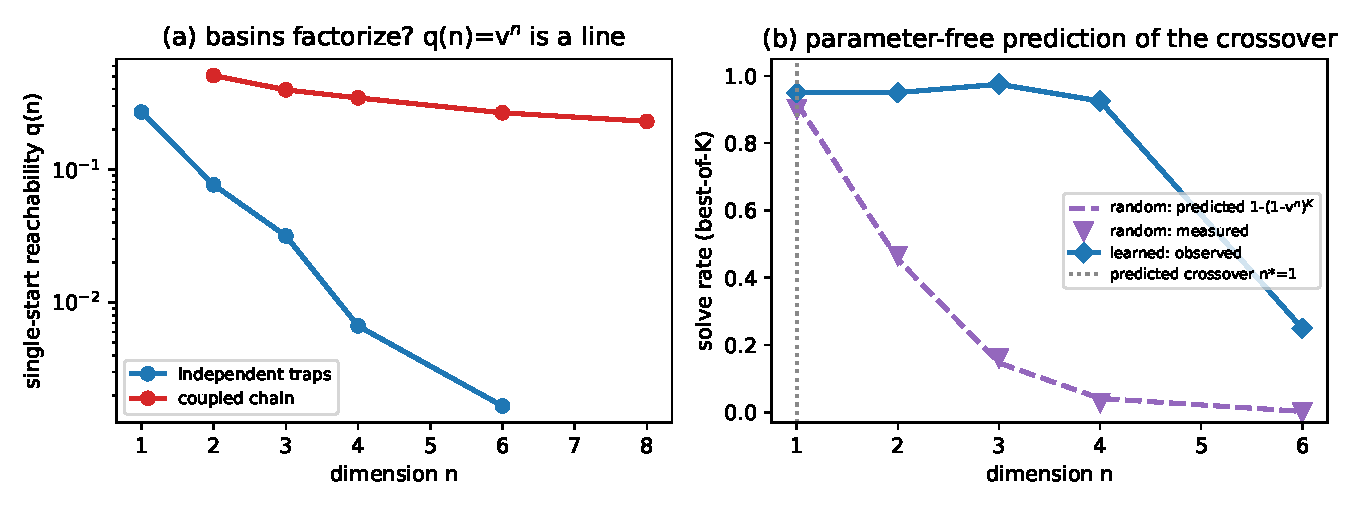
\includegraphics[width=\linewidth]{../figures/fig_crossover_theory.pdf}
\caption{The factorization law, measured. Left: $\log q(n)$ against $n$. The separable family
is a line (slope $-1.03$, $R^2 = 0.98$), the coupled bilinear family is nearly flat
($-0.13$), and the geometry family, though syntactically coupled, collapses ($-0.77$,
$R^2 = 0.999$). Right: the best-of-8 random-restart curve predicted parameter-free from
$v = 0.27$ via Eq.~\eqref{eq:bestofk}, against the measured curve (MAE 0.012), with the
learned hybrid's observed solve rate overlaid; the dotted line is the crossover dimension
predicted from $v$ and the learned ceiling.}
\label{fig:law}
\end{figure}

The separable family behaves exactly as the law requires. $\log q(n)$ is linear with slope
$-1.03$ ($R^2 = 0.98$; the slope alone would imply $v = e^{-1.03} = 0.36$, so the decay is
close to but not perfectly exponential). The parameter-free prediction uses the directly
measured $v = q(1) = 0.27$: substituting that single constant into
Eq.~\eqref{eq:bestofk} reproduces the entire best-of-8 random-restart curve with no free
parameters: predicted 0.919, 0.454, 0.147, 0.042, 0.003 against the measured 0.902, 0.467,
0.162, 0.030, 0.002 at $n = 1, 2, 3, 4, 6$, a mean absolute error of 0.012
% provenance: RESULTS.md R9 + crossover_law.md §5 (crossover_theory.json)
(Figure~\ref{fig:law}). These rates re-measure the random control of Table~\ref{tab:scaling}
at $N = 600$ rather than $N = 40$; the more precise values, 0.90 then 0.47 at $n = 1, 2$, if
anything move the crossover earlier, and they do not change the mechanism. The budget-fair
way to read the dichotomy is the expected number of restarts $1/q(n)$: it explodes from 3.7
to 600 over the separable dimensions while staying between 2.0 and 4.3 on the coupled family.
Any fixed restart budget is therefore exhausted on the separable family, and random search
must eventually lose to a proposal whose ceiling stays comparatively flat. On the coupled
family random search never collapses, a finite crossover dimension does not exist, and a
learned proposal has nothing to amortize. We do not claim a sharp crossover at a particular
$n$; the robust, predicted quantity is the geometric collapse of the restart cost against the
learned ceiling, and the coupled negative that follows is the law's other prediction.

Separability is sufficient for geometric collapse but not necessary, so the diagnostic is the
measured slope, not the syntactic label. A coupled system can still have a steeply decaying
$q(n)$ if each local subproblem admits several basins and errors compound down the chain. A
real-valued geometric domain makes this concrete: chains of unknown points $P_1, \dots, P_k$
($n = 2k$ coordinates) with squared-distance constraints to fixed anchors and between
consecutive points, a genuinely non-convex quartic energy whose solutions the checker accepts
exactly. The family is syntactically coupled, yet its reachability collapses: slope $-0.77$
($R^2 = 0.999$), with $q(n) = 0.653$, 0.147, 0.027, 0.007 at $n = 2, 4, 6, 8$ (150
single-start trials per $n$; its polish is an order of magnitude slower than the synthetic
families' 600)
% provenance: RESULTS.md R9 (geometry) + crossover_law.md §5a
(Figure~\ref{fig:law}, left). Each point's two-circle subproblem has a reflection ambiguity
and spurious basins, so a random start rarely places every point in the right basin, and solve
rates with the classical polish alone are non-saturated (0.56 in-distribution, Wilson
[0.37, 0.73], and 0.28 held out; $N = 25$ per split).
Reachability collapse alone would suggest, by analogy with the separable family, that an
amortized proposal should win here. We tested that prediction by training a denoiser on the
point-chain family with the identical R5 protocol (per-length inline $x_0$ training, one-shot
proposal, the same geometry polish, best-of-8, Checker gate). It does not hold: the learned
proposal ties random restart at every chain length and collapses with it (both 0.625, 0.175,
0.025, 0.000 at $n = 2, 4, 6, 8$, $N = 40$ per length; zero of four significant wins,
$p = 0.50$ each)
% provenance: RESULTS.md R9 (geometry) + PROVENANCE R25 (pointchain_learned.json)
. The negative is the informative result, because it separates two conditions the independent
family had conflated. Reachability collapse (condition one, read off the slope) determines
whether random search fails; it does here. Separability (condition two) determines whether the
denoiser has per-variable marginals to amortize; geometry fails it, because each point's
coordinates are pinned only jointly through the chain. The corrected law needs both: a learned
proposal beats classical search iff reachability collapses \emph{and} the solution is
per-variable separable. The separable traps have both and learning wins; the coupled bilinear
family fails the first, random survives, and learning ties; geometry satisfies the first but
fails the second, and learning ties random and collapses with it. The slope diagnoses random's
behavior, but only separability lets a learned proposal exploit the collapse, so geometry
pins down that collapse is necessary but not sufficient.

\subsection{Coupling removes the advantage}
\label{sec:coupled}

The law of Section~\ref{sec:law} predicts where the crossover must disappear: when acceptance
basins do not factorize, $q(n)$ stays nearly flat, random restart never collapses, and a
learned proposal has nothing to amortize. The test is the coupled chained-bilinear family,
$x_i + x_{i+1} = s_i$ and $x_i \cdot x_{i+1} = p_i$, whose solution is a joint object and
whose measured reachability slope is $-0.13$ (Table~\ref{tab:law}), so what follows is a
prediction checked, not an unexplained negative. Table~\ref{tab:coupled} reports best-of-8
with 60 test instances per $n$.

% provenance: RESULTS.md R7
\begin{table}[t]
\centering
\caption{Coupled chained-bilinear systems (best-of-8, 60 test per $n$). The learned proposal
records zero significant wins over random restart in five comparisons.}
\label{tab:coupled}
\begin{tabular}{ccccl}
\toprule
$n$ & Langevin & random restart & learned & learned $>$ random? \\
\midrule
2 & 0.167 & 0.483 & 0.233 & no (loses) \\
3 & 0.100 & 0.600 & 0.533 & no \\
4 & 0.050 & 0.517 & 0.517 & no (tie) \\
6 & 0.000 & 0.367 & 0.333 & no \\
8 & 0.000 & 0.467 & 0.483 & no \\
\bottomrule
\end{tabular}
\end{table}

The outcome is decisive. The learned proposal ties or loses to random restart at every
dimension, 0 significant wins out of 5. The high-dimensional advantage of
Section~\ref{sec:scaling} was an independence artifact: it required per-variable-separable
solutions the model can memorize as marginals, and it required random restart to collapse
because it must hit all $n$ basins by chance. Under coupling neither condition holds, and the
learned diffusion proposal provides no advantage over random search plus refinement. We regard
this as the most important table in the paper, because it is the boundary of the claim.

\subsection{Relocating the learned component: structural repair beats its controls}
\label{sec:repair}

Coupling closes the route in which the network predicts continuous values, but it does not
exhaust what a learned component can contribute. The one decision the classical solvers cannot
make is discrete and prior to any solve: \emph{which} structure-changing augmentation turns an
unsolvable graph into a solvable one. We move learning there. A candidate-conditioned ranker
applies each of $K$ proposed augmentations, encodes the resulting polynomial graph with
operator-aware node and edge features that expose degree, linear/square/cross participation,
and constants, and scores the augmented graphs listwise; the highest-scoring repair receives
one classical solve and the exact checker remains the acceptance gate. A matched candidate-only
control sees the same augmentation recipe but no problem graph, and \texttt{random} chooses
uniformly among the same $K$ candidates. The predecessor policy classified menu slots over a
single fixed graph encoding and fell to chance on an unseen pattern; the architectural change
that matters is \emph{candidate conditioning} --- encoding each candidate-augmented graph rather
than the fixed graph once. An ablation locates the signal: masking the operator-identity
features (degree, cross/square participation at factor and edge level) and retraining leaves
the ranker essentially intact ($0.981$ vs.\ $0.997$ nonlinear, $0.379$ vs.\ $0.339$ linear),
so the compatibility signal these menus carry lives chiefly in constants, coefficient
magnitudes, and incidence read \emph{jointly with the candidate}, not in the operator flags
per se; we retain the full featurization but do not attribute the gain to it.

% provenance: RESULTS.md R10 + PROVENANCE R20--R24; results/p_repair (Data Version 8)
\begin{table}[t]
\centering
\caption{Candidate-conditioned repair ranker against a candidate-only control and random
selection, on three generalization tests (Data Version 8, Wilson 95\% CIs). Nonlinear menus
carry exact CAS no-real-roots certificates for their distractors; every arm is graded by the
same reference solver that certified the data. The ranker clears both controls on every row;
transfer to an unseen relation is positive but partial.}
\label{tab:repair}
\begin{tabular}{lccc}
\toprule
Test & ranker & candidate-only & random \\
\midrule
Balanced nonlinear ($N{=}360$)          & \textbf{0.997} & 0.333 & 0.236 \\
Vieta $\to$ unseen relation ($N{=}150$) & \textbf{0.420} & 0.120 & 0.253 \\
Linear, unseen pattern ($N{=}400$)      & \textbf{0.380} & 0.195 & 0.287 \\
\bottomrule
\end{tabular}
\end{table}

Table~\ref{tab:repair} reports the three tests that probe generalization. The protocol
(Data Version 8) is deliberately strict: one reference solver certifies the data, grades every
arm, and runs the end-to-end solves; nonlinear ``exactly one solvable option'' is an exact CAS
theorem (a distractor proven to have no real solution is unsolvable at any budget); gold and
distractor parameters share one support and one prior, so whatever surface-form signal survives
is capped at the candidate-only ceiling and anything above that ceiling must come from reading
the problem graph. On the balanced nonlinear test that ceiling is $0.333$ (Wilson 95\% CI
[0.29, 0.38], $N{=}360$) --- above the $0.25$ chance floor, far below the ranker. On balanced
nonlinear menus the ranker reaches $0.997$ against $0.236$ for random, with an exact paired
McNemar test giving $p = 3.3\times10^{-83}$ (274 ranker-only correct versus 0 random-only);
against the candidate-only control the same test gives $p = 1.1\times10^{-72}$ (239 versus 0).
Transfer to an unseen nonlinear relation is positive but partial and holds in both
directions ($0.420$ against $0.253$ for vieta-trained on quad\_link, $0.393$ against $0.180$
for the reverse; $N{=}150$ each), not relation-level invariance. On an unseen linear pattern
the ranker reaches $0.380$ against $0.287$ ($N{=}400$), and rotating the held-out pattern
gives $0.407$ (offset) and $0.450$ (coupled) against $\sim$$0.23$ random, so the effect is not
specific to one holdout choice; over all $1{,}200$ linear test instances it reads
$0.339$ against $0.249$ for random ($p = 7.8\times10^{-7}$, exact paired McNemar). The linear signal is deliberately reported at its post-audit size: closing each
discovered shortcut lowered it ($0.565 \to 0.445 \to 0.380$ across data versions) while pushing
the candidate-only control to chance, so what remains is entirely problem-graph reading — modest
where every operator is linear, decisive on certificate-grade nonlinear menus. Both headline rows
were retrained across three optimization seeds (11, 29, 47) with independent per-seed
evaluation draws: the nonlinear result is optimization-robust ($0.982 \pm 0.006$). The linear
edge is not seed-stable ($0.317 \pm 0.069$, one seed at $0.227$ below the random arm's
$0.248 \pm 0.002$), consistent with reading the linear rows as mechanism evidence rather than
a deployable margin.

% provenance: paper/figures/fig_repair.pdf (scripts/plot_repair.py), RESULTS.md R10
\begin{figure}[t]
\centering
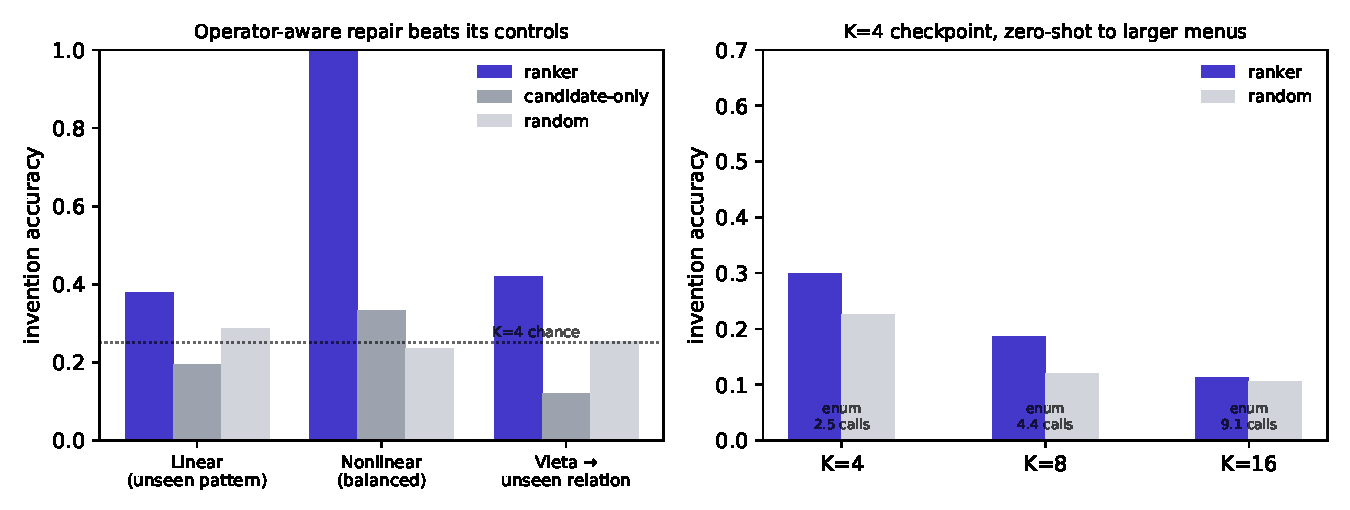
\includegraphics[width=\linewidth]{../figures/fig_repair.pdf}
\caption{Structural repair, measured. Left: the operator-aware ranker against its candidate-only
and random controls on the three generalization tests of Table~\ref{tab:repair}; the dotted line
is $K{=}4$ chance. Right: the $K{=}4$ checkpoint evaluated zero-shot at larger menus retains an
accuracy edge at $K{=}8$ that closes by $K{=}16$, while the blind enumeration it displaces grows
from $2.5$ to $9.1$ solver calls per instance.}
\label{fig:repair}
\end{figure}

The learned component is also cheap where value diffusion was not: one forward pass per
candidate rather than a reverse-diffusion rollout. End to end, applying the selected repair and
invoking the reference solver, the nonlinear ranker's single call solves $0.933$ --- exactly the
oracle and enumeration ceiling --- where blind enumeration averages $2.62$ calls ($N{=}60$);
linear $K{=}4$ solves $0.300$ against $0.227$ random with a $1.000$ ceiling ($N{=}300$). A
cheap-probe control bounds the claim from the other side: spending a short-budget solver call
on every candidate solves at most $0.881$ of nonlinear menus at $4.7$ calls per instance,
where the ranker's single call solves $0.939$ ($N{=}360$; the same checkpoint replayed on the
full probe-suite test split, hence the small offset from the $N{=}60$ end-to-end $0.933$) ---
learning beats probing on accuracy and cost at once,
because provably rootless distractors cannot be ``solved'' at any budget while short probes do
miss the gold. On linear menus the same probe saturates ($0.99$ at $4.4$ calls) and enumeration
is already perfect at $2.5$, so the linear rows are evidence of mechanism, not a deployment
case. The $K = 4$
checkpoint transfers to larger linear menus without retraining, but the accuracy advantage
shrinks with $K$ and is gone by $K = 16$ ($0.300/0.187/0.113$ against random
$0.227/0.120/0.107$ at $K = 4/8/16$, $N = 300/150/150$); what survives at large $K$ is only the cost gap, as the enumeration it
displaces grows to $9.05$ solver calls per instance (Figure~\ref{fig:repair}, right). Directly
training at $K = 16$ performs at chance, so the transferred checkpoint is selected and both
negatives are kept in the record. The scope is menu-based repair on synthetic factor graphs;
``exactly one solvable option'' is an exact certificate for all linear menus (rank) and $99\%$
of nonlinear test menus (CAS real-root nonexistence), with the remainder carrying a disclosed
budget-relative probe certificate.

\subsection{External validity: standard real systems}
\label{sec:real}

Every family above is procedurally generated, so we also ran the solver battery on eight
recognized test problems encoded once as factor graphs: two-circle and conic--line
intersections, GPS-style trilateration, the Rosenbrock and Himmelblau stationary-point systems,
two- and three-link inverse kinematics, and the cyclic-4 computer-algebra benchmark. Their real
roots are irrational, so acceptance is a numeric residual tolerance ($\max_j |r_j(x)| < 10^{-6}$),
the fair criterion for comparing numerical solvers.
% provenance: RESULTS.md R26 + real_systems.md (results/p_real/real_systems.json)
The result reinforces the paper's boundary on problems we did not construct. Multi-start
Levenberg--Marquardt solves all eight; annealed Langevin solves one and random restart with the
gradient polish solves four. Where the gradient polish fails --- the Rosenbrock valley, the
Himmelblau saddles, the overdetermined trilateration basin, the six-variable 3R chain, all with
single-start reachability $0.00$ --- a stronger \emph{classical} polish (LM) fixes every case,
so the bottleneck there is the finisher, not the proposal, and a learned proposal would inherit
the same weak polish. No system in the suite falls in the amortization regime the law identifies:
these problems are low-dimensional and coupled, so classical search suffices, exactly as the
factorization law predicts for real coupled systems. This is external validity for the
characterization, not a new positive: the learned component is not run per system, because a
suite with one instance per structure offers nothing to amortize.

\subsection{Scope: what these problems are, and are not}
\label{sec:scope}

All families above are synthetic and procedurally generated. To locate MARC's paradigm against
real problem text we measured coverage on a 48-problem sample of MATH-500
\citep{hendrycks2021math}: the template formalizer covers 0 of 48 problems. By hand
classification, roughly 20\% of the sample is constraint-shaped (MARC's paradigm), about 31\%
is CAS computation, and about 48\% is reasoning or proof, outside the architecture's scope.
The binding constraint is autoformalization from natural language to constraint graphs, not
the solver. MARC targets continuous algebraic constraint solving; it does not do general
mathematical reasoning, and we report this coverage number so the scope is quantified rather
than implied.\footnote{The learned structural component is the candidate-conditioned repair
ranker of Section~\ref{sec:repair}. Its predecessor, a discrete-diffusion slot policy, produced
preliminary numbers that were withdrawn (evaluation seeds overlapped the validation seeds used
for checkpoint selection), and those are not cited here; the ranker is evaluated under the
disjoint-seed Data Version 8 protocol, which also withdrew the earlier v6/v7 ranker numbers
after a pin-prior leak and probe-artifact distractor certificates were found and fixed.}
% provenance: RESULTS.md R6 (prose); footnote provenance: RESULTS.md R8/R10

\section{Limitations}
\label{sec:limitations}

The central limitation is the one the coupled experiment establishes: the learned proposal's
advantage requires per-variable-separable solutions and a regime where random restart
collapses, and on coupled systems it ties or loses to random multi-start at every dimension
tested. We believe the cause is structural rather than a matter of tuning; the denoiser
effectively learns per-variable marginals, so any joint solution space removes the advantage.
Even on the favorable independent families the model gains nothing at $n = 1$ (random restart
is at ceiling) and degrades to 0.250 at $n = 6$, so the useful window is the crossover region,
not high dimension in general.

The factorization law carries its own caveats. Eq.~\eqref{eq:bestofk} uses the
instance-averaged $q$; per-instance reachability varies, so best-of-$K$ computed from the
average is an approximation (a Jensen gap), and we validate the parameter-free prediction
against a best-of-$K$ curve self-measured under identical conditions rather than against a
separate experiment. The learned proposal's ceiling is measured, not derived: the law predicts
the random-restart curve and the collapse of the restart cost, not the learned model's
absolute accuracy, and it says nothing about the capacity-limited decay at $n = 6$. And while
the reachability prediction is validated on three families, the solve-rate consequence is
confirmed on the separable positive, the coupled negative, and now geometry, where a trained
denoiser ties random restart and collapses with it: reachability collapse turned out to be
necessary but not sufficient, and the geometry test corrected our initial reading that the
slope alone flags a domain as learning-favorable.

Several failures are specific and reportable. CircleLine is never solved by the learned
proposal: 0.000 in-distribution against 0.200 for random restart, and 0.000 in cross-family
transfer. Transfer succeeds on only two of four held-out families, and adding CircleLine to a
training mix collapsed an otherwise recoverable transfer (0.70 to 0.00), so a bad training
family actively hurts. The entrapment result, while pre-registered and precise, is
confirmatory: annealed Langevin escaping deterministic traps is textbook behavior, and we
claim measurement on this substrate, not novelty. The predecessor structure policy (a
discrete-diffusion slot classifier) never separated from random selection and its numbers
remain withdrawn; the candidate-conditioned ranker of Section~\ref{sec:repair} replaces it
under the Data Version 8 protocol. Within that result, the linear edge is not stable across
optimization seeds ($0.317 \pm 0.069$, one seed below the random arm), so only the nonlinear
headline ($0.982 \pm 0.006$) is optimization-robust and the linear rows stand as mechanism
evidence only. Finally, the synthetic-family boundary has two measured exceptions: the
geometry domain of Section~\ref{sec:law} enters at both the reachability and the solve-rate
level (its learned arm ties random restart and collapses with it), and the real-systems suite
of Section~\ref{sec:real} is solve-rate but classical-arms only; the MATH coverage measurement
(0/48) quantifies how far the current formalizer is from real problem text.

\section{Conclusion}
\label{sec:conclusion}

We set out to test whether a learned diffusion proposal helps solve continuous algebraic
constraint systems, and we ran the control that decides the question. The outcome is a
characterization. The propose-and-polish recipe is genuinely better than cold-start Langevin
refinement on trapped non-convex families, but the proposal need not be learned there. The
learned proposal earns its place only where search is independent across variables and
dimension defeats random restart, a regime we can exhibit cleanly at $n \ge 3$, and this
advantage disappears under coupling. The factorization law compresses that characterization
into one measured quantity, the single-start reachability slope, and reproduces the
random-restart curve it predicts without a fitted parameter. These boundaries close the route
from learned value proposals to a general claim over classical search on this problem class. What survives is the
substrate (exact symbolic residuals, energy guidance, and an exact checker wrapped around any
proposer) and the division of labor it supports. The decision classical solvers cannot make is
not which values to try but which structure to add, and that is exactly where the learned
component earns its place: the certificate-grade repair ranker of Section~\ref{sec:repair}
clears every control it faces, on menus where "exactly one solvable option" is a theorem
rather than a budget-relative claim.

\bibliographystyle{plainnat}
\bibliography{refs}

\end{document}
